\index{domain completeness!limitations}
The verification approach to solve the domain completeness problem in \cref{sec-dc-verification,thm:C-extensionCompleteness} is defined under the following assumptions which are likewise the limitations of the presented approach:

\begin{enumerate}
  \item The conditions for verifying domain completeness are only sufficient but not necessary.
  \item The approach is only applicable to graph grammars with empty start graphs.
  \item The approach is only applicable to graph grammars with non-deleting productions.
  \item The approach only involves constraints that are designated for general satisfaction while neglecting constraints that are designated for initial satisfaction.
  \item Constraints and application conditions need to be in $\M$-normal form.
  \item Termination of the approach requires an upper bound.
\end{enumerate}

\subsection{Conditions are Sufficient but not Necessary}

The conditions for verifying domain completeness in \cref{thm:C-extensionCompleteness} are only sufficient but not necessary.
Consider a grammar $\GG$ with duplicates of creating productions but for which the domain completeness holds.
The duplicates lead to a non-$C$-conflict-freeness of the marking rules $m(\GG)$ when claiming critical pairs of same rules and same matches.
Thus, the condition does not hold.
However, it is simple to exclude duplicates from the grammar.
For the confluence of marking rules we can find a similar example.

\subsection{Graph Grammars with Non-Empty Start Graph}

\begin{figure}[!tb]
\begin{center}
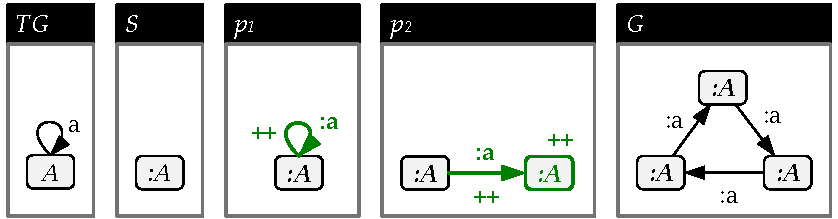
\includegraphics[width=.68\textwidth]{img/limitations/startgraph.pdf}
\end{center}
\caption{Limitation: Graph Grammar with Non-Empty Start Graph $S$}
\label{fig:sec-dc-general-lim:startgraph}
\end{figure}

We assume graph grammar $\GG=(S,P)$ typed over type graph $\TG$, with start graph $S$ and productions $P=\{p_1,p_2\}$ as depicted in \cref{fig:sec-dc-general-lim:startgraph}.
Furthermore, we assume that the set of domain constraints $C=\varnothing$ is empty.
By \cref{def:C-extensionCompleteness}, $\Lang(\GG)$ is $C$-extension complete and furthermore, by \cref{def:cf-marking-rules} $m(\GG)$ is $C$-conflict free, i.e., the conditions in \cref{sec-dc-verification,,thm:C-extensionCompleteness} hold.
However, for graph $G$ in \cref{fig:sec-dc-general-lim:startgraph} we obtain that $G \in \Lang(C)$ but $G \not\in \Lang(\GG)$.
Therefore the language inclusion does not hold although the conditions for domain completeness hold.
This is due to the gap between the declarative nature of graph constraints and the constructive nature of graph grammars.
Thus, the approach is only applicable to graph grammars with empty start graphs.

\subsection{Graph Grammars with Deleting Productions}

\begin{figure}[!tb]
\begin{center}
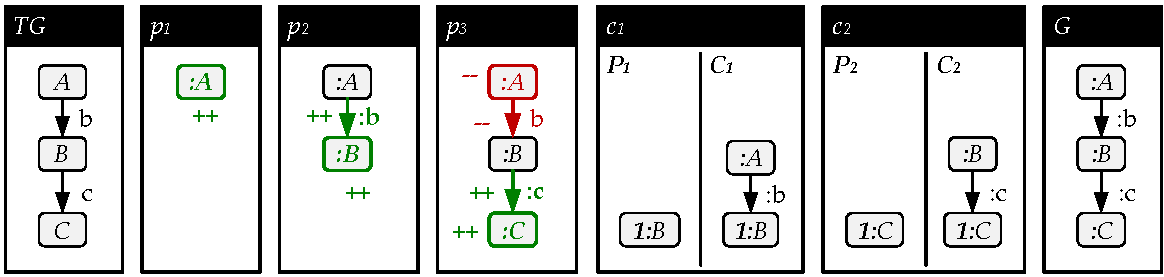
\includegraphics[width=\textwidth]{img/limitations/deleting.pdf}
\end{center}
\caption{Limitation: Graph Grammar with Deleting Production $p_3$}
\label{fig:sec-dc-general-lim:deleting}
\end{figure}

We assume graph grammar $\GG=(S=\varnothing,P)$ typed over type graph $\TG$ with the empty start graph and productions $P=\{p_1,p_2,p_3\}$ as depicted in \cref{fig:sec-dc-general-lim:deleting}.
Furthermore, we assume the set of domain constraints $C=\{c_1\colon P_1 \to C_1,c_2\colon P_2 \to C_2\}$ as depicted in \cref{fig:sec-dc-general-lim:deleting}.
Note that $\Lang(\GG)$ is $C$-extension complete by \cref{def:C-extensionCompleteness} and $m(\GG)$ seems to be $C$-conflict free by \cref{def:cf-marking-rules} when neglecting the deleting elements in production $p_3$.
Therefore, the conditions for domain completeness in \cref{sec-dc-verification,,thm:C-extensionCompleteness} seem to hold.
However, for graph $G$ in \cref{fig:sec-dc-general-lim:deleting} we obtain that $G \in \Lang(C)$ but $G \not\in \Lang(\GG)$.
Therefore the language inclusion does not hold.
This is due to the definition of marking rules which are only defined for non-deleting productions.
The example shows that elements that are deleted via productions cannot simply be neglected in marking rules.
Thus, the approach cannot be trivially extended to graph grammars with deleting productions and is only applicable to graph grammars with non-deleting productions.

\subsection{Initial \& General Satisfaction}
\begin{figure}[!tb]
\begin{center}
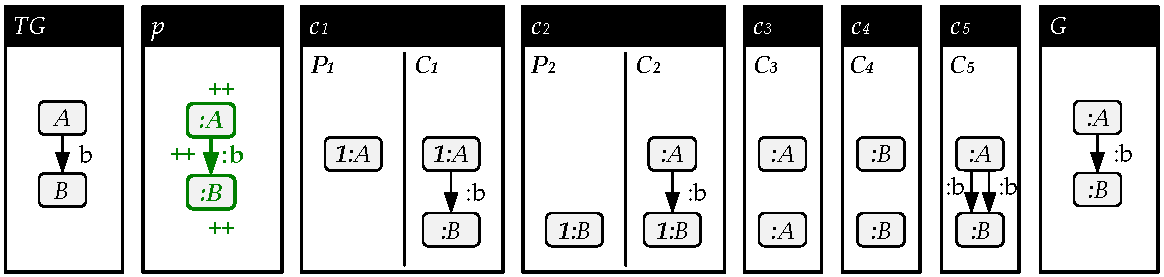
\includegraphics[width=\textwidth]{img/limitations/general.pdf}
\end{center}
\caption{Limitation: Initial \& General Satisfaction}
\label{fig:sec-dc-general-lim:igsat}
\end{figure}

Given type graph $\TG$, constraints $C_G=\{c_3,c_4\}$ designated for general satisfaction and $C_I=\{c_1,c_2\}$ designated for initial satisfaction, and grammar $\GG=(\varnothing,\{p\})$ where $c_1=\exists(P_1 \to C_1,\true),c_2=\exists(P_2 \to C_2,\true),c_3=\neg\exists(\varnothing \to C_3,\true),c_4=\neg\exists(\varnothing \to C_4,\true)$ and $c_5=\neg\exists(\varnothing \to C_5,\true)$.
Note that $\Lang(C)=\{G\} \subseteq \Lang(\GG)$, i.e., domain completeness holds.
However, constraints $c_1$ and $c_2$ are not used for $C$-extensions in \cref{sec-dc-verification,def:C-extension}, since, both are designated for initial satisfaction.
Therefore, $C$-extension completeness of $\Lang(\GG)$ does not hold, since, effective atoms $P_1,P_2$ and $G$ are not extended and cannot be created via grammar $\GG$.
The approach may be extended to also involve constraints that are designated for initial satisfaction in future work in order to handle situations from above appropriately.

\subsection{Constraints \& Application Conditions in $\M$-normal Form}

% \begin{figure}[!tb]
% \begin{center}
% 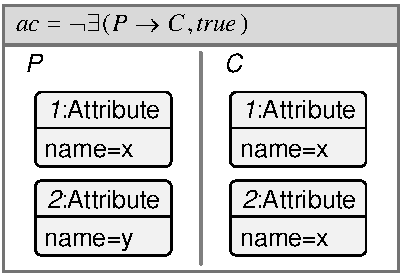
\includegraphics[width=.37\textwidth]{img/limitations/constraint.pdf}
% \end{center}
% \caption{Limitation: Application Condition not in $\M$-normal Form}
% \label{fig:sec-dc-general-lim:nf}
% \end{figure}

Note that for domain completeness, the graphs in $\Lang(C)$ and $\Lang(\GG)$ share the same ``concrete" algebra up to isomorphism by general assumption of \cref{sec-dc-verification}.
For verifying domain completeness $\Lang(C) \subseteq \Lang(\GG)$ in \cref{sec-dc-verification,,thm:C-extensionCompleteness}, we assume that all constraints $C$ and all application conditions in productions of graph grammar $\GG$ need to be in $\M$-normal form.
This is due to the fact that domain completeness is verified only once on the level of the $\DSIG$-term algebra for the data part and domain completeness for all concrete algebras can then be implied by \cref{sec-dc-verification,lem:ac_schema_sat_inst_mor,lem:atiti} but only when assuming the restriction to conditions in $\M$-normal form.
Therefore, a verification for each case of concrete algebras is not necessary.
\cref{sec-dc-verification,ex:schema_sat} depicts the necessity for conditions in $\M$-normal form and the full proof of \cref{sec-dc-verification,thm:C-extensionCompleteness} reveals all details.
In contrast to the presented approach, when performing the domain completeness verification directly on the concrete algebra for each case instead of a verification on the more abstract level of the term-algebra, then the restriction to conditions in $\M$-normal form may be loosened in future work.
Note that the restriction to conditions in $\M$-normal form forbids the definition of conditions that identify elements on the data part.
Therefore, constraints and application conditions of the following form cannot be expressed: ``For two or more nodes that have a node attribute $x$ each, it holds that all attributes $x$ share the same attribute value''.
However, we are confident that conditions in $\M$-normal form have enough expressive power for real-world scenarios.
% Consider the negative application condition $\ac=\neg\exists(P \to C,\true)$ in \cref{fig:sec-dc-general-lim:nf}.
% The NAC is not in $\M$-normal form, since, variables $x$ and $y$ are both mapped to $x$.
% A production in grammar $\GG$ that is equipped with this NAC is only applicable to graphs via matches, if the two matches \code{Attribute}s have different \code{name}s.
% However, the extension over atoms are only formed via $\M$-morphisms in \cref{def:C-extension} - Therefore, the construction does not lead to extension where both names share the same variable.
% Therefore, the language inclusion is verified on the abstract level of the term algebra, i.e., terms with variables, for attribute values, whereas graphs with concrete attributes values may identify different variables to the same concrete value, i.e., there may be transformation steps for graphs on the term level but not on the level for corresponding concrete graphs with concrete values.
% Thus, the conditions in \cref{sec-dc-verification} for the language inclusion holds although they may be graph that cannot be created via grammar $\GG$.
% More precisely, for a graph $P'=P[x \mapsto 1,y \mapsto 1]$ which is graph $P$ from \cref{fig:sec-dc-general-lim:nf} but where variables $x$ and $y$ are substituted by concrete value $1$ we obtain $P \models \ac$ but $P' \not\models \ac$.

\subsection{Termination Requires Upper Bound}

According to \cref{th:sec-dc-verification:term_dc}, we have to define an upper bound for the size of graphs in order to ensure termination of the approach.
In most cases, the verification terminates without restricting to an upper bound.
However, when restricting to an upper bound we could also check for all graphs up to the upper bound which satisfy the constraints in $C$ if they can be created via the rules in grammar $\GG$ for ensuring the validity of language inclusion $\Lang(C) \subseteq \Lang(\GG)$.
On the other hand, the verification via C-extension completeness in \cref{thm:C-extensionCompleteness} may be more efficient, since, not all graphs need to be checked but rather a small subset.
